\documentclass[pmlr]{jmlr}
% EAIM 2027 at AAAI -- manuscript prepared from the official template.
% Original syntax examples: eaim-template-reference.tex and eaim-sample.pdf.
% Compile with pdfLaTeX. Keep the template's page layout and typography.
% amsmath, amssymb, natbib, graphicx, url, algorithm2e are loaded by jmlr.
\usepackage{longtable}
\usepackage{booktabs}
\usepackage{siunitx}

\jmlrvolume{YYY} % Assigned by the organisers upon acceptance.
\jmlryear{2027}
\jmlrworkshop{EAIM2027 at AAAI}
\editors{K. Bhandari, S. Zheng, J. Shier, D. Herremans, S. Colton}

% REVIEW VERSION: leave false for every anonymous submission.
% Change to \camerareadytrue only when preparing the identified version.
\newif\ifcameraready
\camerareadyfalse

% Working title; the short running title keeps the page header within the text width.
\title[Sparse Timbre Control of Percussive Audio]{Sparse Timbre Control of Percussive Audio with Joint Modal, Noise, and Transient Synthesis}
\ifcameraready
  % First author: Minjun Kim. Corresponding author: Eunwoo Song.
  \author{\Name{Minjun Kim} \Email{oxymoron@yonsei.ac.kr}\and
    \Name{Eunwoo Song\nametag{\thanks{Corresponding author.}}}
    \Email{eunwoo.song@yonsei.ac.kr}\\
    \addr Department of Electrical and Electronic Engineering, Yonsei University}
\else
  % Preserve the template's two-author anonymous layout.
  % No real names, emails, affiliation, or corresponding-author marker.
  \author{\Name{Anonymous 1}\and
    \Name{Anonymous 2}\\
    \addr Anonymous affiliation}
\fi

\begin{document}
\maketitle

\begin{abstract}
Percussive one-shots range from pitched drums to cymbals with dense modal content, and sound designers often want to adjust the timbre of an existing sample rather than generate a new one.
Differentiable analysis--synthesis models such as DrumBlender reconstruct a given sample through interpretable components, but their low-level parameters offer no high-level control, and their constant-Q analysis struggles with dense high-frequency modes.
This paper builds on DrumBlender and reconstructs a one-shot as the sum of jointly trained modal, noise, and transient components.
Sinusoidal tracks from a hybrid constant-Q and short-time Fourier analysis receive bounded corrections, noise bands following NoiseBandNet are conditioned on the corrected modal parameters, and a small temporal convolutional network adds a transient computed from the modal waveform.
After training, a sparse autoencoder fitted to the shared representation provides label-free controls whose edits start from the reconstruction of the given sample and act through the synthesis parameters.
\textbf{[TBD: one or two sentences on the measured reconstruction and control results.]}
\end{abstract}

\begin{keywords}
differentiable digital signal processing; percussion synthesis; timbre control; modal analysis; sparse autoencoders
\end{keywords}


\section{Introduction}
\label{sec:intro}

% P1. Percussive sound and why sinusoids plus noise fall short.
Percussive sounds are produced by striking vibrating solids such as membranes, bars, plates, and shells, and their timbre varies widely with the shape, size, and material of the struck object \citep{fletcher1998physics}.
Because the instrument vibrates freely after the strike, these sounds share a decaying envelope. 
Modeling and synthesis of percussive audio date back to analog drum machines such as the Roland TR-808 \citep{werner2014physically,werner2014tr808} and have been approached through physical modeling \citep{bilbao2010percussion}, signal processing \citep{karplus1983digital}, and, most recently, neural audio synthesis (NAS), in which deep generative models learn to synthesize drum sounds from data \citep{aouameur2019neural,drysdale2020adversarial,nistal2020drumgan,rouard2021crash}.
Spectral modeling synthesis (SMS) \citep{serra1990spectral} represents a sound as sinusoidal partials with slowly varying amplitudes and frequencies \citep{mcaulay1986speech} plus a stochastic residual, and differentiable digital signal processing (DDSP) \citep{engel2020ddsp} implements a synthesizer of this kind with differentiable operations, so that a neural network can be trained end to end to predict its parameters from audio while each synthesis module keeps an interpretable role.
Applied to percussion, this formulation represents the modes of the struck body as sinusoids and the remainder as stochastic noise, which suits instruments with a clear pitch and prominent modes, such as membranophones.
For tom-toms, a mode-wise analysis and synthesis based on the discrete cosine transform has even produced samples that listeners could not distinguish from recordings \citep{kirby2021evolution}.
Idiophones such as cymbals, in contrast, consist of hundreds or even thousands of modes that give them a noisy high-frequency range, and their sound blooms as the vibration moves from linear to nonlinear regimes \citep{skare2019realtime,chaigne2005nonlinear}, which makes them difficult to analyze.
The strike itself also produces a short broadband burst, the \textit{transient}, so a percussive sound combines narrow-band components with components that change rapidly over time, and neither is easily captured by sinusoids and noise alone \citep{verma2000extending,barahonarios2024noisebandnet}.

% P2. Differentiable responses to these difficulties and the remaining problem.
DDSP has since been adopted in a wide range of synthesis approaches \citep{hayes2024review,shan2022differentiable,caspe2022ddx7,barahonarios2024noisebandnet}, including several that extend it to inharmonic sounds \citep{renault2023ddsp,diaz2023rigid,hayes2023sinusoidal}.
Transients have likewise been given a dedicated component, both in classical sines, transients, and noise representations \citep{levine1998sines,verma2000extending} and in differentiable models \citep{liu2024ddspsfx,simionato2025sines}.
DrumBlender \citep{shier2023differentiable} brought this sines, noise, and transient decomposition to percussion, yet cymbals remained the hardest class to reconstruct.
With a limited set of sinusoidal tracks, much of the dense modal content of a cymbal is left for the stochastic noise component, so a single model that reconstructs both pitched drums and cymbals faithfully remains difficult.

% P3. Timbre control and the gap.
Reconstruction alone, however, does not give a sound designer a way to change a sound.
Percussion synthesis has offered timbre control through the fixed circuits of analog drum machines \citep{werner2014physically,werner2014tr808} and through timbral descriptors and latent spaces of neural drum generators \citep{aouameur2019neural,ramires2020neural,nistal2020drumgan,lavault2022stylewavegan}.
Outside percussion, control has also been obtained from latent spaces learned without timbre labels \citep{caillon2021rave,kotowski2026plaud,paek2025learning}.
An analysis--synthesis model such as DrumBlender \citep{shier2023differentiable} reconstructs a given sample through interpretable parameters, but these parameters are low-level and numerous, and high-level control was left as future work.
Turning these parameters into high-level timbre controls requires controls that are learned without labels, start from the reconstruction of the given sample, and act through the parameters of the synthesizer.

% P4. This work.
To this end, this paper builds on DrumBlender \citep{shier2023differentiable} and reconstructs a percussive one-shot as the sum of modal, noise, and transient components, which are trained jointly through their summed output.
The modal component starts from sinusoidal tracks obtained by a hybrid of constant-Q transform (CQT) and short-time Fourier transform (STFT) analysis, and a neural network predicts bounded corrections to their frequencies and amplitudes.
The noise component is a bank of narrow noise bands following NoiseBandNet \citep{barahonarios2024noisebandnet}, whose amplitudes are predicted with the corrected modal parameters as an additional input, and a small temporal convolutional network adds a transient computed from the modal waveform, which makes the model a hybrid of signal processing and neural synthesis.
After reconstruction training, a sparse autoencoder (SAE) is fitted to the shared representation of the frozen model, and its temporal features define continuous edits around the reconstruction of each sample.
These edits are evaluated on held-out one-shots, together with the separate effects of the modal-to-noise and transient conditioning paths.
Trained on about 17,000 one-shots collected from public datasets and commercial sample packs, the model \textbf{[TBD: reconstruction result relative to DrumBlender]}, and its SAE features provide controls that \textbf{[TBD: control result]}.

The contributions of this paper are as follows.
\begin{itemize}
  \item A hybrid modal analysis front-end that tracks both low-frequency modes and dense, short-lived high-frequency modes (\sectionref{sec:method-analysis}).
  \item A jointly trained modal, noise, and transient synthesizer in which bounded corrections refine the analyzed tracks and the noise and transient components are conditioned on the corrected modal component to model unlabeled diverse percussive audio (\sectionref{sec:method-synthesis}).
  \item Sample-anchored timbre controls from a post-hoc temporal SAE, with separate interventions to measure how a latent edit propagates through modal conditioning of noise and the transient clip code (\sectionref{sec:method-control}).
\end{itemize}


\section{Related Work}
\label{sec:related}

% B1. Signal models, modal analysis, and differentiable percussion models.
\paragraph{Analysis and synthesis of percussive sound.}
Signal models of drum sounds predate deep learning, as in the drum variant of the Karplus--Strong algorithm, which turns a noise burst into an unpitched decaying sound \citep{karplus1983digital}.
Modal approaches instead describe a drum as a set of decaying modes derived from recordings or measurements.
\citet{kirby2021evolution} modeled the pitch glide of each mode of a tom-tom across strike intensities, and \citet{nagata2025sound} synthesized drum sounds from transfer functions obtained by experimental modal analysis.
These models reproduce a particular instrument closely, but they are built from that instrument rather than learned across a heterogeneous sample library.
Differentiable modal synthesis learns such parameters from data, for example by predicting differentiable modal resonators from the shape, material, and strike position of an object \citep{diaz2023rigid}.
Learning the frequencies themselves is harder, because the loss surface over sinusoidal frequency is non-convex and contains many local minima \citep{hayes2023sinusoidal}.
In DDSP-Piano, a second training phase that fine-tunes the inharmonicity and detuning parameters, among others, did not improve the perceived quality in a listening test \citep{renault2023ddsp}.
In DrumBlender, the sinusoidal frequencies are therefore not learned but extracted before training by peak tracking on a constant-Q transform, and the noise and transient parameters are predicted by encoders adapted from the convolutional encoder of the SoundStream codec \citep{shier2023differentiable,zeghidour2022soundstream}.
For stochastic components, NoiseBandNet predicts the time-varying amplitudes of a bank of narrow noise bands \citep{barahonarios2024noisebandnet}.
In contrast, this work applies a hybrid constant-Q and short-time Fourier analysis to every instrument class in a sample library, keeps the analyzed tracks and their initial phases, and learns only bounded corrections of their frequencies and amplitudes.
Its noise bands follow NoiseBandNet, but their amplitudes are predicted jointly with the modal corrections and conditioned on them, and its transient component restricts the modal-driven TCN of DrumBlender to the modal waveform and a single clip-level code.

% B2. Generative drum models and the controls they expose.
\paragraph{Neural drum synthesis and its controls.}
Beyond the descriptor-conditioned models discussed in \sectionref{sec:intro}, neural drum synthesis has explored several generative families and forms of control.
\citet{drysdale2020adversarial} conditioned a WaveGAN-based model on the drum class and explored its latent space by interpolation.
StyleWaveGAN adapts a style-based generator to raw waveforms and combines discrete drum-type control with continuous perceptual descriptors and per-class amplitude envelopes \citep{lavault2022stylewavegan}.
CRASH applies score-based diffusion directly to raw audio and can regenerate an existing sound from its latent code under a deterministic sampler \citep{rouard2021crash}.
In a user study of a style-based drum generator, unsupervised latent directions were rated slightly higher than random and supervised ones, although not significantly \citep{ramires2022study}.
\citet{drysdale2024latent} explored the latent space of a drum generator through latent arithmetic, dimensionality reduction, and visualization.
\citet{waissbluth2022synthesis} instead reconstructed snare drum samples as sparse mixtures of a small fixed sample library with a variational autoencoder, so that moving through its latent space swaps samples in and out of the mixture.
In these systems, an existing sample can be edited only through the generator's own representation of it, obtained by an encoder or by inversion \citep{nistal2022drumganvst,rouard2021crash}, so the edit applies to the generator's approximation of the sample.
In contrast, this work starts from the given recording, reconstructs it with modal, noise, and transient components whose parameters are derived from an analysis of that recording rather than from a fixed library, and applies the controls to that reconstruction.

% B3. Learned latent spaces and controls without labels.
\paragraph{Label-free control of learned audio representations.}
Neural audio codecs learn compact latent representations for high-fidelity reconstruction \citep{zeghidour2022soundstream,kumar2023high}, but their latent dimensions are not trained to correspond to perceptual attributes.
Variational autoencoders impose a prior that makes the latent space easier to traverse, and \citet{esling2018generative} further aligned latent distances between instrument classes with perceptual timbre spaces, which requires instrument labels and human dissimilarity ratings.
Sparse autoencoders offer a post-hoc alternative that reconstructs the activations of a trained model through a wide layer of sparsely active features \citep{gao2025scaling}.
Such features have been identified in audio latent spaces \citep{paek2025learning} and used to steer large generative music models \citep{singh2026discovering}.
For percussion, \citet{shier2024realtime} learned without parameter supervision to map onset features of acoustic snare hits to parameter changes of a differentiable TR-808-style snare synthesizer.
\citet{shier2025designing} extended this timbre remapping to non-differentiable synthesizers and reported that the temporal morphology of a hit, namely how its loudness and spectrum evolve over time, was poorly mapped.
In contrast, this work fits a sparse autoencoder post hoc to the shared representation of a frozen model that reconstructs a given sample, so that label-free edits reach the modal and noise components through their synthesis parameters.


\section{Method}
\label{sec:method}
\begin{figure}[t]
\floatconts
  {fig:overview}
  {\caption{Overview of the proposed model. The analyzed tracks $P_0$ and the waveform encoder feed the shared representation $h$, from which the modal corrections $\hat{P}$, the noise-band amplitudes $a_b$, and a clip code $\mathbf{s}$ for the transient TCN are predicted. Dashed lines mark the stop-gradient input of the TCN and the post-hoc SAE edit of $h$, during which $\mathbf{s}$ keeps its unedited value.}}
  {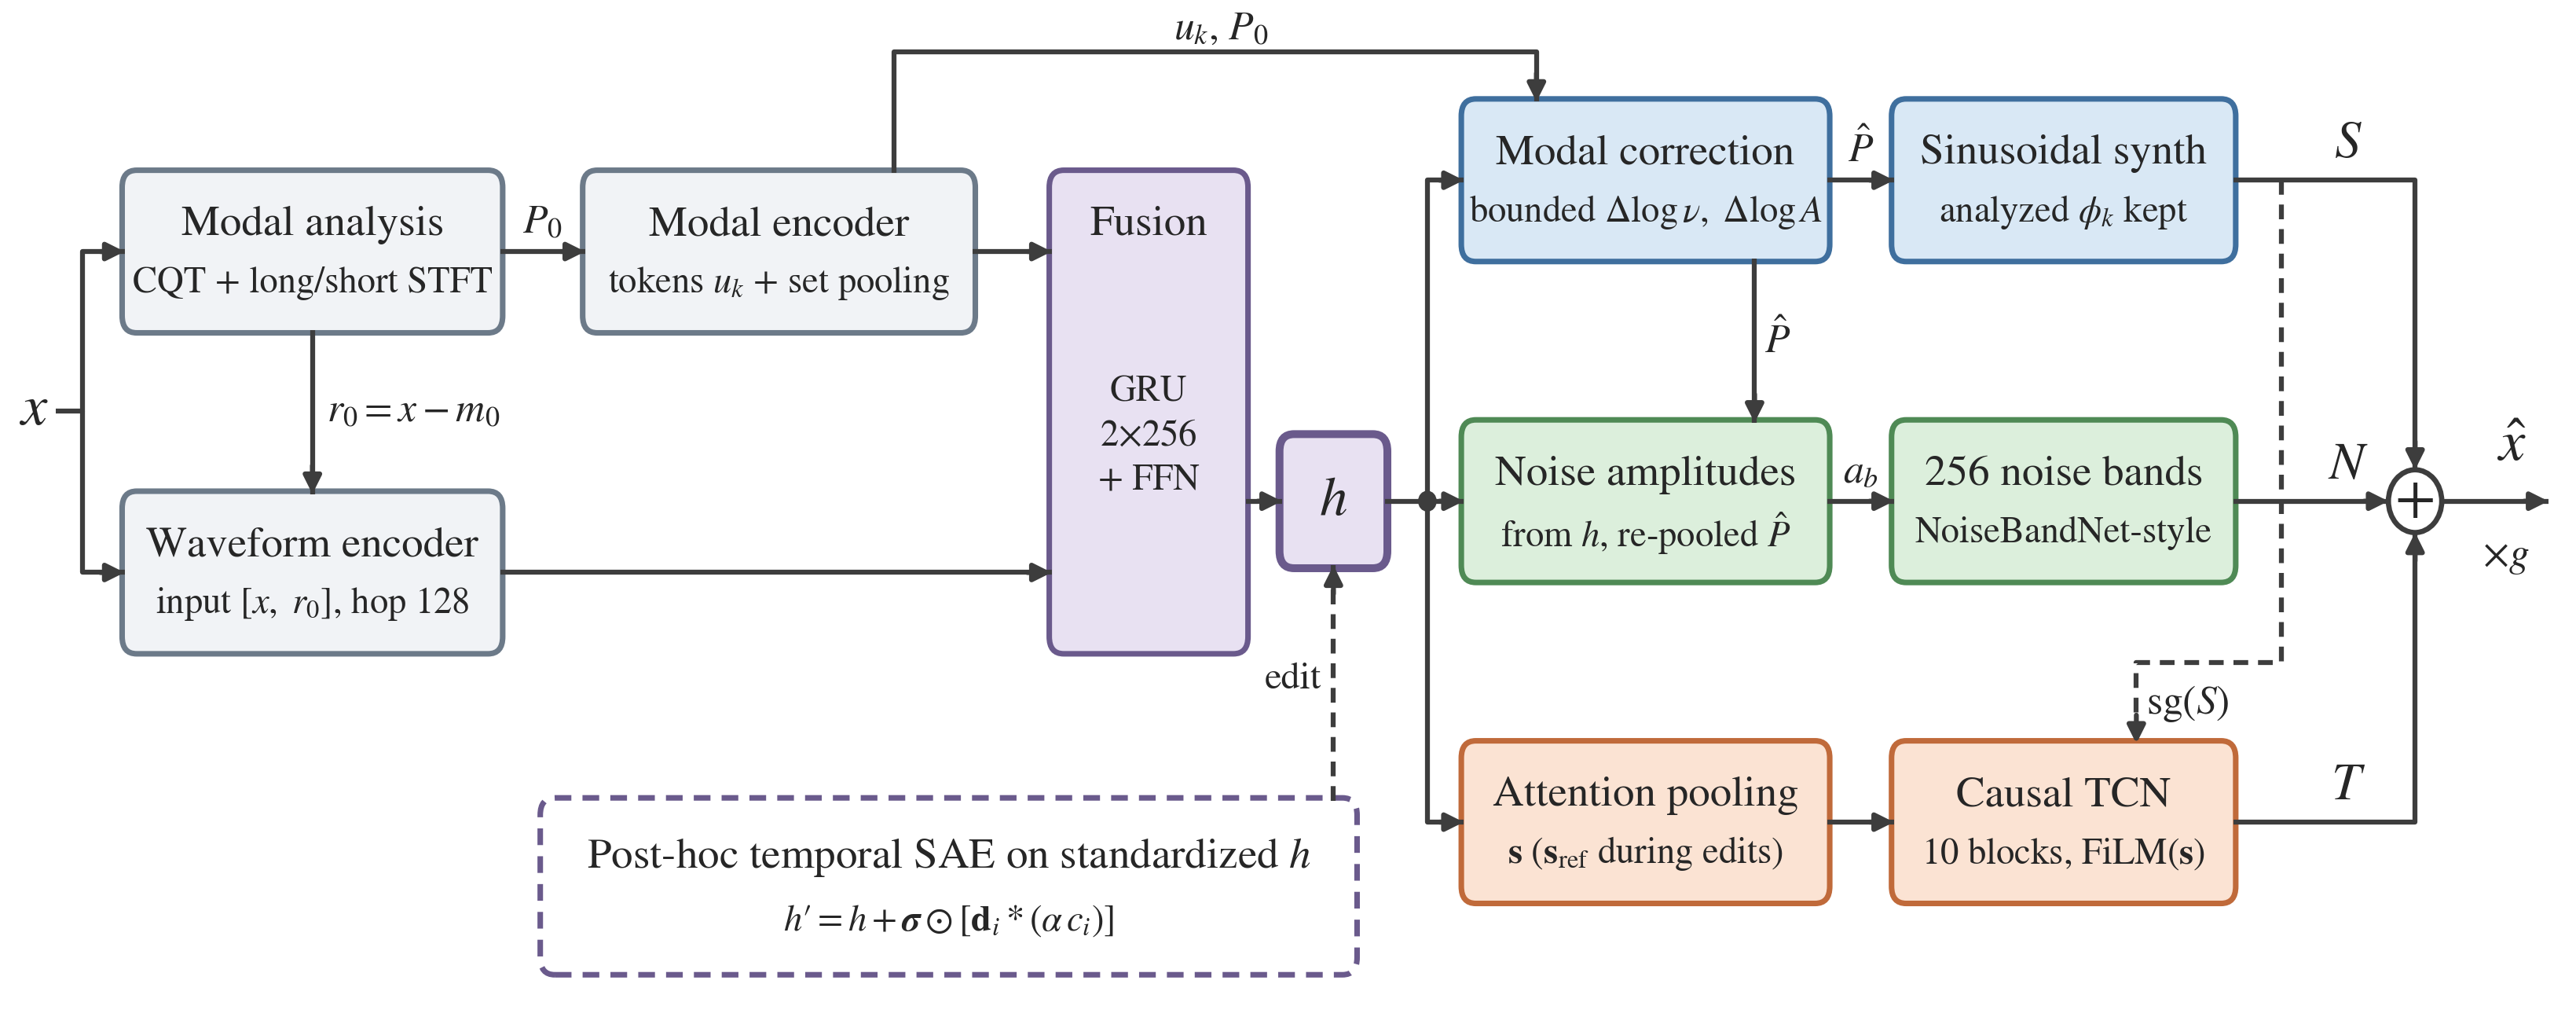
\includegraphics[width=\linewidth]{figures/figure1.png}}
\end{figure}
The proposed model reconstructs a percussive one-shot $x$ as
\begin{equation}
\hat{x} = g\,(S + N + T),
\label{eq:model}
\end{equation}
where $S$, $N$, and $T$ are the modal, noise, and transient components and $g$ is a gain shared by all three.
$S$ and $N$ are rendered by signal processing synthesizers from parameters predicted by a neural network, whereas $T$ is generated by a small TCN.
All three components are driven by one shared representation and are trained jointly through their sum, and label-free controls are later obtained from an SAE fitted to this representation.
\figureref{fig:overview} summarizes the analysis, the shared representation, the three synthesis paths, and the point at which the controls act.
The model builds on DrumBlender \citep{shier2023differentiable}: it keeps the three-component decomposition, the waveform encoder, and the modal-driven TCN, revises the modal analysis, and replaces the filtered noise with the noise bands of NoiseBandNet \citep{barahonarios2024noisebandnet}.
Signals are sampled at 48~kHz.

\subsection{Modal Analysis and Reference}
\label{sec:method-analysis}
Each sample is first analyzed into sinusoidal tracks that serve as the reference for the modal component.
DrumBlender applies the peak picking and parabolic interpolation of sinusoidal analysis \citep{serra1990spectral} to a CQT and keeps up to 64 tracks.
The CQT resolves low-frequency resonances well, but its bins widen with frequency, from about 1.8~Hz at 60~Hz to about 29~Hz at 1~kHz with 24 bins per octave.
More critically, its tracker links peaks greedily from the tail toward the onset with a tolerance of 5\% of the CQT bin index, which at 1~kHz admits any peak between about 820 and 1220~Hz and widens further at higher frequencies, so distinct peaks, such as an early peak at 1~kHz and a later one at 850~Hz, can be joined into a single gliding track.
Because DrumBlender extracts these tracks before training and renders them without correction, such merged tracks go directly into the output, where their gliding frequencies produce artifacts and the energy they wrongly assign to the modal component distorts what the noise and transient components must model.

This work therefore keeps the CQT only below 700~Hz and adds full-band STFTs whose long window resolves frequency and whose short window localizes short-lived resonances in time.
Peaks are refined by parabolic interpolation of the log magnitude \citep{smith1987parshl}, and overlapping peaks are fitted jointly.
Tracks are linked by one-to-one matching within a frequency range predicted from each track, with a cost on phase continuity.
Short or weak tracks are discarded, and at most 64 tracks are kept.
The result is a reference parameter set $P_0=\{\nu_k[j], A_k[j], \phi_k\}$ with frequency $\nu$ in cycles per sample, amplitude $A$, and initial phase $\phi_k$ for track $k$ and analysis frame $j$.

The waveform and the reference amplitudes are divided by the peak absolute value $g$ of $x$, so that the relative levels of the components are preserved when the output is rescaled in \equationref{eq:model}.
The reference modal waveform $m_0$ is rendered from $P_0$, and the reference residual is $r_0=x-m_0$; both are fixed for each sample.
The residual is given only to the waveform encoder and is not a target for the noise or transient components, because correcting the modal parameters changes which part of $x$ the modal component leaves unexplained.

\subsection{Shared Representation}
\label{sec:method-encoder}
A waveform encoder, which follows the convolutional encoder of SoundStream \citep{zeghidour2022soundstream} used in DrumBlender, receives $x$ and $r_0$ as two channels and produces one frame every 128 samples (2.67~ms at 48~kHz).
A modal encoder embeds the frequency, amplitude, and initial phase of each track and frame with a shared perceptron and processes each track along time without mixing tracks, which yields per-track tokens $u_k[j]$.
Because a track index does not refer to the same mode across samples and each token already carries its frequency and amplitude, these tokens are also summarized in each frame by attention pooling with learned queries, following the Set Transformer \citep{lee2019set}. 
The waveform features and the pooled modal context are fused and passed through a two-layer gated recurrent unit (GRU) \citep{cho2014learning} and feed-forward blocks, similar to the DDSP decoder \citep{engel2020ddsp}, to produce the shared representation $h$.
No skip connection bypasses $h$, so every learned audio feature reaches the synthesizers through $h$, which makes $h$ the single point at which the controls act.

\subsection{Synthesis Components}
\label{sec:method-synthesis}
\paragraph{Modal component.}
A correction head shared by all tracks reads each token $u_k[j]$ together with $h$ and predicts two values $q^{\mathrm{f}}_k[j]$ and $q^{\mathrm{a}}_k[j]$, which are mapped to bounded multiplicative corrections,
\begin{equation}
\hat{\nu}_k[j]=\nu_k[j]\exp\!\big(0.03\tanh q^{\mathrm{f}}_k[j]\big),\qquad
\hat{A}_k[j]=A_k[j]\exp\!\big(\log(4)\tanh q^{\mathrm{a}}_k[j]\big).
\label{eq:modal-correction}
\end{equation}
The frequency is thus corrected by at most about $\pm 52$ cents and the amplitude by a factor between $1/4$ and $4$, and the head is initialized so that the modal component initially reproduces the reference.
The corrected set is denoted by $\hat{P}=\{\hat{\nu}_k[j], \hat{A}_k[j], \phi_k\}$.
Frequency is corrected only locally because the loss surface over sinusoidal frequency is non-convex \citep{hayes2023sinusoidal}.
The correction cannot create new track.
With the parameters interpolated to audio rate and $n$ indexing samples, the modal component is
\begin{equation}
S[n]=\sum_{k}\hat{A}_k[n]\sin\!\Big(\phi_k+2\pi\sum_{m=0}^{n}\hat{\nu}_k[m]\Big),
\label{eq:modal-synth}
\end{equation}
where the initial phase $\phi_k$ stays at its analyzed value and the subsequent phase follows the corrected frequency.

\paragraph{Noise component.}
Following NoiseBandNet, the noise component is a sum of 256 fixed narrow bands with time-varying amplitudes,
\begin{equation}
N[n]=\sum_{b=1}^{256} a_b[n]\,\xi_b[n+o_b],
\label{eq:noise}
\end{equation}
where $\xi_b$ is a precomputed band-limited noise signal, read circularly from an offset $o_b$ that is random during training and fixed during evaluation, and $a_b$ is the amplitude of band $b$.
The bands are spaced linearly up to 6~kHz and logarithmically above.
The amplitudes are predicted from $h$ together with $\hat{P}$, which is summarized again with the perceptron and pooling of the modal encoder, so the noise component depends on the modal correction and its gradient also reaches that correction.

\paragraph{Transient component.}
The transient component keeps the modal-driven TCN of DrumBlender but restricts its inputs to
\begin{equation}
T=\mathrm{TCN}\big(\mathrm{sg}(S);\,\mathbf{s}\big),
\label{eq:transient}
\end{equation}
where $\mathrm{sg}$ denotes the stop-gradient operator and $\mathbf{s}$ is a single 16-dimensional vector per clip obtained by attention pooling of $h$.
The TCN consists of ten causal dilated convolution blocks with a receptive field of about 43~ms.
Each block is modulated by feature-wise linear modulation (FiLM) \citep{perez2018film} with coefficients computed once from $\mathbf{s}$, and the output layer is initialized to zero so that $T=0$ at the start of training.
Because its input is stopped, $T$ cannot pull the modal parameters through $S$, and the restriction biases $T$ toward a correction of the modal waveform without guaranteeing that it contains only the attack.

\subsection{Training Objective}
\label{sec:method-training}
The model is trained from scratch on the reconstruction of the summed output in \equationref{eq:model} with
\begin{equation}
\mathcal{L}=\mathcal{L}_{\mathrm{spec}}+\lambda_{\mathrm{env}}\,\mathcal{L}_{\mathrm{env}},\qquad \lambda_{\mathrm{env}}=0.1.
\label{eq:loss}
\end{equation}
The spectral loss is the multi-resolution STFT loss of Parallel WaveGAN \citep{yamamoto2020parallel} over four STFT sizes $M\in\{256,1024,4096,8192\}$ with Hann windows and hop $M/4$,
\begin{equation}
\mathcal{L}_{\mathrm{spec}}=\frac{1}{4}\sum_{M}\left(\frac{\lVert \hat{X}_M-X_M\rVert_F}{\lVert X_M\rVert_F}+\big\langle\,\lvert\log\hat{X}_M-\log X_M\rvert\,\big\rangle\right),
\label{eq:spec-loss}
\end{equation}
where $X_M$ and $\hat{X}_M$ are the magnitude spectrograms of the target and the reconstruction, $\langle\cdot\rangle$ denotes the mean over time-frequency bins, and both spectrograms are computed on the valid extent of each sample.
The small STFT sizes resolve the attack in time, whereas the large ones separate closely spaced modes in frequency.
The envelope loss $\mathcal{L}_{\mathrm{env}}$ is the mean absolute difference between the log RMS levels of the target and the reconstruction over 128-sample frames.
Whereas the spectral loss compares individual time-frequency bins, this term compares the overall level of each frame, so that the onset and the decay rate are constrained.

\subsection{Label-Free Controls}
\label{sec:method-control}
After reconstruction training, the model is frozen, and its shared representation $h$ is cached for each one-shot.
The channels are standardized with the mean $\boldsymbol{\mu}$ and standard deviation $\boldsymbol{\sigma}$ of the valid training frames, each weighted by the fraction of the frame occupied by audio.
A temporal SAE reconstructs this standardized representation, with a temporal convolution and frame-wise TopK activation \citep{gao2025scaling} in its encoder and unit-norm temporal atoms in its decoder.

For a reference sample, the sparse code $\mathbf{c}$ is computed once.
A knob multiplies the activation sequence $c_i$ of feature $i$ by $1+\alpha$, which gives the edited code $\mathbf{c}'$, and with decoder $D$ and atom $\mathbf{d}_i$ the edit is
\begin{equation}
\begin{aligned}
h' &= h + \boldsymbol{\sigma}\odot\big[D(\mathbf{c}')-D(\mathbf{c})\big] \\
   &= h + \boldsymbol{\sigma}\odot\big[\mathbf{d}_i * (\alpha c_i)\big],
\end{aligned}
\label{eq:edit}
\end{equation}
where $*$ is convolution over time and $\odot$ rescales the channels.
Because only the change of the decoder output is added, the reconstruction error of the SAE does not enter the edit, and every knob starts from the reconstruction of the given sample, which is returned directly at $\alpha=0$.
The TopK selection of the reference is kept fixed during a sweep, and the edit has no effect on clips in which $c_i$ is zero.

The default edit recomputes the modal corrections and noise amplitudes from $h'$ while keeping the reference clip code $\mathbf{s}_{\mathrm{ref}}$, so the transient responds only through the edited modal waveform.
For analysis, a joint-plus-strike render also recomputes $\mathbf{s}$ from $h'$ while reusing the edited modal and noise waveforms, and a strike-only render applies the same change of $\mathbf{s}$ with the neutral modal and noise waveforms.
All renders share the reference gain and noise offsets.


\section{Experiments}
\label{sec:experiments}

\subsection{Dataset}
\label{sec:exp-data}
The dataset combines two public percussion datasets, MDLib2.2 \citep{prockup2013toward} and the Dynamic Percussion Dataset \citep{nieminen2020dynamic}, with free and commercial sample packs, including packs from Splice.
It covers acoustic drum kits with many kinds of cymbals and hi-hats, electronic drums from a wide range of genres, tuned and world percussion such as marimbas, vibraphones, steelpans, and bells, and a smaller share of found-object and foley hits.
Every sample is a one-shot containing a single strike.
In total, about 17,000 samples are used.
Each sample pack is split into training, validation, and test sets in a ratio of 80/10/10.

\subsection{Baseline}
\label{sec:exp-baseline}
The baseline is DrumBlender \citep{shier2023differentiable}, retrained from scratch on the same data, whose output is $\hat{x} = S + T(S) + N$.
Here, $S$ is rendered from 64 sinusoidal tracks extracted by peak tracking on a CQT, $T$ is a TCN applied to $S$ and conditioned through FiLM on the embedding of a SoundStream encoder \citep{zeghidour2022soundstream}, and $N$ is white noise shaped by time-varying filters whose magnitudes are predicted by a second SoundStream encoder.
The original implementation trains on fixed-length clips, so it is adapted to complete clips of up to 20~s with the zero-padded part excluded from the loss, and indexing errors in its CQT tracker are fixed, while its synthesizers, encoders, and multi-resolution STFT loss are otherwise unchanged.

\subsection{Training}
\label{sec:exp-train}
Both systems are trained with Adam \citep{kingma2015adam} at an initial learning rate of $10^{-4}$, which is halved when the validation loss stops improving, and training stops early when the validation loss no longer improves, after at most 150 epochs.
Both systems use an effective batch size of 32 through gradient accumulation, and the proposed model additionally clips the gradient norm at 1.0.

\paragraph{Post-hoc SAE training.}
The SAE uses 512 atoms, TopK with $K=8$, and nine-frame encoder and decoder kernels, and it is trained with Adam at a learning rate of $3\times10^{-4}$ on batches of 16 crops.
Each crop contains 256 core frames with eight context frames on each side, and the loss is evaluated on the valid core frames.
The loss is a valid-frame-weighted mean squared error plus an AuxK term with weight $1/32$ \citep{gao2025scaling}, which fits the detached main residual with up to 128 features that have not been active in the last $10^6$ valid core frames and starts after the first such window.
The checkpoint with the lowest validation reconstruction error is kept, the validation rate of dead features is reported separately, and SAE training is limited to three hours.

\subsection{Evaluation}
\label{sec:exp-eval}
Reconstruction is evaluated on the test set over the valid, unpadded extent of each clip, and lower is better for all metrics.
The multi-resolution STFT distance (MR-STFT) sums spectral convergence and log-magnitude distance at three resolutions \citep{yamamoto2020parallel}, as implemented in auraloss \citep{steinmetz2020auraloss}; these are the resolutions of the baseline's training loss.
The log-spectral distance (LSD) is the root-mean-square difference between frame-wise log power spectra, computed as in the DrumBlender implementation.
To examine high-frequency content separately, the LSD is also computed with a 4096-point STFT in the bands below 250~Hz, from 250~Hz to 4~kHz, and above 4~kHz.
The spectral flux onset error (SF) is the mean absolute difference between the onset-strength signals of the output and the target, each obtained by squaring and summing the half-wave rectified increase in STFT magnitude between frames.
Scores are computed per file and summarized by their mean and standard deviation over the test set.
% Also computed but not reported: log-RMS envelope error (1024-sample frames, hop 256; close to the proposed model's envelope loss) and MFCC error (40 coefficients without c0, 128 mel bands).

\subsection{Control Evaluation}
\label{sec:exp-control}
Between 8 and 12 SAE features are shortlisted by their activation coverage across validation clips and source packs.
Each shortlisted feature is auditioned on three active validation one-shots at $\alpha\in\{-1,0,1\}$, with the clip, reference gain, and noise offsets shared within each triplet and the listening copies level-matched.
Up to two features are selected as knobs whose audible variations remain useful when the one-shot is played as a rhythmic hit, and features with weak responses are also auditioned at $\alpha=+2$ and $+4$, with these extrapolative edits reported separately.
Before the test set is evaluated, the atom indices, the primary render scope, and one descriptor with its direction of change are fixed for each knob on the validation set.

On held-out clips, each knob is swept over $\alpha\in\{-1,-0.5,0,0.5,1\}$ with the reference gain, and the evaluation reports the coverage of active clips, the median and interquartile range of the descriptor change, and the agreement with the validation direction, after checking that $\alpha=0$ reproduces the neutral render.
The modal edit is examined by comparing the neutral and edited modal waveforms, alone and mixed with the reference noise and transient, including the amplitude and frequency changes of tracks with appreciable energy.
To isolate the modal conditioning of the noise component, $h'$ and the noise offsets are held fixed while the reference and edited modal summaries are swapped, and the resulting change is reported relative to the neutral noise level.
To isolate the clip code, the joint and joint-plus-strike renders are compared with identical modal and noise waveforms, and their transients are compared after fitting a single gain, with the remaining attack and tail differences reported.

As a matched null, fixed random signed channel permutations are applied to the actual latent change, which preserves its frame-wise norm and temporal inner products, following the matched-norm comparison of \citet{singh2026discovering}.
Time-invariant band gains are also fitted to the edited-versus-neutral log spectrum, and the remaining time-dependent change indicates how much of an edit a static equalizer cannot reproduce.
Audio examples illustrate the knob trajectories on repeated strikes of the same sample.


\section{Results and Discussion}
\label{sec:results}
\subsection{Reconstruction}
\label{sec:results-recon}
% Table tab:reconstruction-evaluation currently lists two checkpoints (epoch036-step00015910 and epoch047-step00020640) per sample pack; state which system they belong to and which checkpoint is reported.
% Compare with the DrumBlender baseline on the same test files, per pack.
\textbf{[TBD: reconstruction results.]}
\begin{table*}[t]
\centering
\caption{Test-set reconstruction errors. Values are per-file mean $\pm$ standard deviation.}
\label{tab:reconstruction-evaluation}
\footnotesize
\setlength{\tabcolsep}{4pt}
\begin{tabular}{llrccc}
\hline
Run & MR-STFT $\downarrow$ & LSD $\downarrow$ & SF $\downarrow$ \\
\hline
DrumBlender & $1.524 \pm 0.407$ & $2.661 \pm 0.756$ & $23.407 \pm 140.719$ \\
 % & Pack A & 61 & $1.400 \pm 0.185$ & $2.963 \pm 0.289$ & $0.336 \pm 0.709$ \\
 % & Pack B & 6 & $1.626 \pm 0.184$ & $3.003 \pm 0.327$ & $2.665 \pm 3.173$ \\
 % & Pack C & 1046 & $1.372 \pm 0.291$ & $2.265 \pm 0.212$ & $0.386 \pm 1.330$ \\
 % & Pack D & 379 & $1.753 \pm 0.456$ & $3.312 \pm 0.909$ & $70.100 \pm 255.428$ \\
 % & Pack E & 13 & $1.791 \pm 0.141$ & $2.818 \pm 0.257$ & $12.209 \pm 19.002$ \\
 % & Pack F & 62 & $2.090 \pm 0.607$ & $3.818 \pm 1.412$ & $167.107 \pm 313.117$ \\
 % & Pack G & 57 & $1.843 \pm 0.473$ & $3.280 \pm 0.794$ & $43.742 \pm 105.810$ \\
 % & Pack H & 32 & $1.968 \pm 0.150$ & $3.278 \pm 0.206$ & $8.925 \pm 12.560$ \\
 % & Pack I & 72 & $1.639 \pm 0.160$ & $2.918 \pm 0.317$ & $1.963 \pm 3.272$ \\
\hline

\end{tabular}
\end{table*}

\subsection{Controls}
\label{sec:results-control}
\textbf{[TBD: control results.]}

\subsection{Analysis Front-End}
\label{sec:results-analysis}
% Optional ablation: CQT-only versus hybrid tracks under the same synthesis model.
\textbf{[TBD: whether this ablation is run.]}

\subsection{Limitations}
\label{sec:results-limitations}
% Candidates: within-pack split only; noncausal analysis (the 20 Hz CQT observes about 1.7 s); not a real-time plugin; tracks are explanatory sinusoids, not physical modes.
\textbf{[TBD: limitations.]}


\section{Conclusion}
\label{sec:conclusion}
% Drafted before the final runs; check each claim against the measured results.
This paper presented a model for percussive one-shots that builds on DrumBlender and reconstructs a given sample as the sum of modal, noise, and transient components.
Its modal tracks come from a hybrid CQT and STFT analysis and receive bounded corrections, its noise bands are conditioned on the corrected modal parameters, and its transient is computed from the modal waveform and a clip-level conditioning code.
Trained on about 17,000 one-shots from public datasets and commercial sample packs, the model \textbf{[TBD: reconstruction result relative to DrumBlender]}.
A post-hoc SAE defines sample-anchored timbre edits from the shared representation without timbre labels.
The evaluation measures their held-out effects and isolates how modal conditioning and the transient clip code contribute to the edited sound, and \textbf{[TBD: control result]}.
Future work includes a listening study of the controls, a causal analysis front-end for real-time use, and noise bands of different lengths that avoid repetition in long tails.


% Add any required generative-AI disclosure accurately in Method or here.
% Identity-revealing acknowledgements belong only in the camera-ready version:
% \ifcameraready
% \acks{...}
% \fi

% Keep verified BibTeX entries in eaim.bib; use \citep{key} or \citet{key}.
\bibliography{eaim}

%\appendix
%\section{Additional Details}
\label{apd:details}
% TODO: add supplementary material when available.


% Template conventions:
% - Figures/tables: \floatconts{label}{\caption{...}}{contents}, [htbp].
% - References: \sectionref, \figureref, \tableref, \equationref.
% - Use jmlr's \subfigure; avoid conflicting caption/subcaption packages.
% - Main text: 8--11 pages excluding references (official CFP, 2026-10-29).
% - Review PDF and public links must not reveal author identities.
% - Do not submit source containing the camera-ready author block unless allowed.
\end{document}
